\documentclass[12pt,a4paper]{article}

\usepackage[utf8]{inputenc}
\usepackage[T1]{fontenc}
\usepackage[brazilian]{babel}
\usepackage{graphicx}
\usepackage{amsmath,amssymb,amsthm}
\usepackage{booktabs}
\usepackage{float}
\usepackage{geometry}
\usepackage{caption}
\usepackage{subcaption}
\usepackage{xcolor}
\usepackage{enumitem}
\usepackage[round]{natbib}
\usepackage{array}
\usepackage{multirow}
\usepackage{tabularx}
\usepackage[colorlinks=true,linkcolor=blue,citecolor=blue,urlcolor=blue]{hyperref}
\usepackage{doi}

\geometry{a4paper, margin=2.5cm}

% Ambientes de teoremas (PT-BR)
\theoremstyle{definition}
\newtheorem{pressuposto}{Pressuposto}
\newtheorem{definicao}{Definição}

\theoremstyle{plain}
\newtheorem{lema}{Lema}
\newtheorem{proposicao}{Proposição}
\newtheorem{teorema}{Teorema}
\newtheorem{corolario}{Corolário}

% ============================================================
\title{Dinâmica de Desinformação em Processos Eleitorais:\\
Um Modelo SEIR Baseado em Agentes para Propagação de Fake News\\
e Intervenções de Política Pública%
\thanks{Declarações do autor sobre o Protocolo de Disseminação Pós-Publicação e uso de IA em pesquisa estão no Apêndice~\ref{app:author_statements}.}}

\author{
    Daniel T G N Maciel%
    \thanks{Docente, Programa de Pós-Graduação em Economia, Universidade Federal de Mato Grosso (UFMT), Brasil. E-mail: \texttt{daniel.maciel@ufmt.br}. Autor correspondente.}
}

\date{Abril de 2026}

% ============================================================
\begin{document}

\maketitle

% ============================================================
\begin{abstract}
Este artigo investiga como a desinformação se espalha durante eleições e como três intervenções complementares --- educação midiática, verificação de fatos e regulação de robôs automatizados --- podem contê-la. Usando simulação computacional com 1.000 agentes virtuais (eleitores, influenciadores, robôs e verificadores de fatos) interagindo em redes sociais por 100 dias de campanha eleitoral, calibramos o modelo com 7.200 notícias brasileiras rotuladas e o aplicamos a dez países da América Latina. A principal descoberta é que nenhuma intervenção isolada é suficiente: verificação de fatos, educação midiática e regulação de bots atuam isoladamente como remédios parciais, mas somente juntas reduzem a exposição à desinformação entre 86\% e 93\% em todos os dez países. Mais importante: em 8 dos 10 países, os robôs automatizados são o motor indispensável da epidemia de desinformação --- sem eles, a desinformação não se sustentaria. Venezuela e Bolívia são as duas exceções, onde a transmissão entre pessoas já seria suficiente. Em todos os cenários, a política combinada reduz o alcance da desinformação abaixo do limiar necessário para reverter o resultado de qualquer eleição recente da região.

\vspace{0.3cm}
\noindent\textbf{Palavras-chave:} fake news, modelagem baseada em agentes, SEIR, eleições, redes sociais, política pública, desinformação, América Latina.

\vspace{0.2cm}
\noindent\textbf{Classificação JEL:} C63, D72, D83, L86.
\end{abstract}

% ============================================================
\section{Introdução}
\label{sec:intro}

A desinformação tornou-se um desafio definidor para as democracias contemporâneas. Estudos empíricos em larga escala demonstram que conteúdos falsos se propagam mais rapidamente, alcançam públicos mais amplos e penetram mais profundamente nas redes sociais do que informações precisas \citep{vosoughi2018spread}. Em contextos eleitorais, essas dinâmicas têm consequências particularmente graves: durante a eleição presidencial norte-americana de 2016, notícias falsas pró-Trump foram compartilhadas mais de trinta milhões de vezes no Facebook \citep{allcott2017social}, e até 27,4\% dos eleitores foram expostos a conteúdos de baixa credibilidade \citep{guess2020exposure}. A eleição presidencial brasileira de 2018 trouxe evidência complementar do problema, com o WhatsApp funcionando como vetor primário de disseminação de desinformação, onde imagens falsas superaram as verdadeiras por fator de oito \citep{machado2019whatsapp, resende2019misinformation}. O episódio brasileiro tornou visível uma característica estrutural da América Latina que distingue o problema regional das democracias anglófonas: a coexistência entre plataformas criptografadas de mensageria em grupos fechados e mídias sociais abertas, ambiente no qual a moderação automatizada é estruturalmente limitada e a verificação de fatos depende de infraestrutura social.

Apesar da crescente documentação empírica, a modelagem computacional da desinformação em eleições permanece fragmentada. Modelos epidêmicos clássicos de propagação de rumores \citep{daley1964epidemics, maki1973mathematical} tratam os agentes como homogêneos e ignoram a heterogeneidade cognitiva que determina a suscetibilidade individual \citep{pennycook2021psychology}. Modelos epidêmicos baseados em redes \citep{pastor2001epidemic, newman2002spread} capturam efeitos topológicos sobre os limiares de propagação, mas omitem a dinâmica de opinião e o papel estratégico de contas automatizadas. Modelos de dinâmica de opinião \citep{deffuant2000mixing} abordam a convergência de crenças e a polarização, mas não incorporam a mecânica de transmissão de desinformação. Modelos baseados em agentes de fake news \citep{franceschi2022agent, tornberg2018echo} começaram a integrar alguns desses elementos; contudo, nenhum arcabouço existente combina simultaneamente epidemiologia informacional, heterogeneidade de agentes, topologia de rede, dinâmica de opinião e consequências eleitorais em um único modelo analiticamente fundamentado.

Este artigo aborda essa lacuna. Desenvolvemos um modelo baseado em agentes (MBA) que adapta a dinâmica epidemiológica SEIR à propagação de desinformação ao longo de uma campanha eleitoral simulada de cem dias. O modelo conta com mil agentes heterogêneos --- eleitores, influenciadores, bots de desinformação e verificadores de fatos --- interagindo em uma rede dual que combina uma grade espacial $32 \times 32$ com um grafo livre de escala de Barabási-Albert. Seis cenários de política pública são avaliados em cento e oitenta rodadas de simulação para o Brasil (trinta replicações por cenário), e a análise comparativa entre dez países da América Latina soma 1.800 simulações. Um sistema de equações diferenciais ordinárias de campo médio fornece parâmetros analíticos de referência, enquanto o MBA captura fenômenos emergentes decorrentes da heterogeneidade e da estrutura de rede.

O achado central diz respeito ao número básico de reprodução da desinformação. No Brasil, a transmissão exclusivamente humano-humano produz $R_0^{\text{hum}} \approx 0{,}71 < 1$ no ponto central da calibração, o que significa que, sem contas automatizadas, a desinformação tende a não se sustentar. Os bots elevam o número de reprodução efetivo para $R_0^{\text{eff}} = 30/11 \approx 2{,}73$, produzindo uma epidemia informacional. Somente a intervenção combinada --- educação midiática, expansão da verificação de fatos e regulação de bots --- reduz o pico de infecção em 90,3\% no Brasil e entre 86\% e 93\% nos dez países analisados, levando o número de reprodução sob política combinada a $R_0^{\text{comb}} = 0{,}31$. Aplicando a mesma derivação aos outros nove países, oito deles exibem $R_0^{\text{hum}} < 1$ no ponto central; Venezuela ($\approx 1{,}15$) e Bolívia ($\approx 1{,}02$) são as duas exceções em que a transmissão humano-humano pode se sustentar mesmo na ausência de bots. Interpretamos esse resultado como indicação de que a necessidade de bots para o estado endêmico é \emph{regime-dependente}: empírica na maioria dos contextos, porém não universal.

As contribuições do artigo articulam-se em três eixos. No eixo teórico, oferecemos um arcabouço SEIR informacional de cinco compartimentos com probabilidades de transição moduladas por viralidade do conteúdo, credibilidade da fonte, credibilidade aparente e educação midiática do receptor, acompanhado de dinâmica eleitoral via confiança delimitada de Deffuant-Weisbuch e formalização matemática completa com demonstrações de conservação, positividade, estabilidade do equilíbrio livre de doença via Routh-Hurwitz, convergência de crenças sob exposição repetida e condições analíticas para reversão eleitoral. No eixo computacional, implementamos quatro tipos de agentes cognitivamente heterogêneos sobre rede de camada dupla, comparamos seis cenários de política e documentamos a divergência sistemática de 11,3 pontos percentuais entre a previsão de campo médio e o resultado do MBA, atribuindo-a à heterogeneidade, à topologia da rede e ao comportamento de fonte permanente dos bots. No eixo empírico comparativo, estendemos o arcabouço a dez países latino-americanos --- aproximadamente 88\% da população da região, excluído o Caribe --- e introduzimos um sistema explícito de três níveis de qualidade de dados que torna transparente a incerteza paramétrica, respondendo a preocupações metodológicas levantadas em estudos comparativos recentes \citep{lupu2020socialmedia, waisbord2018post, bradshaw2019global}.

O restante do artigo está organizado como segue. A Seção~\ref{sec:literature} revisa as evidências empíricas e o arcabouço conceitual subjacentes ao modelo. A Seção~\ref{sec:model} descreve o modelo seguindo o protocolo ODD \citep{grimm2010odd}. A Seção~\ref{sec:formalization} apresenta a formalização de campo médio e os números de reprodução, incluindo a derivação específica por país. A Seção~\ref{sec:experiments} detalha o desenho experimental e a parametrização comparativa entre países. A Seção~\ref{sec:results} reporta os resultados para o Brasil e para a comparação entre os dez países, bem como a divergência entre campo médio e MBA. A Seção~\ref{sec:discussion} discute implicações de política pública; a Seção~\ref{sec:limitations} registra limitações e extensões futuras; e a Seção~\ref{sec:conclusion} apresenta as conclusões. Todas as derivações analíticas foram verificadas de forma independente com SymPy (Python) e Wolfram Language; os scripts e os dados de replicação estão arquivados em repositório persistente com DOI atribuído no momento da submissão.

% ============================================================
\section{Desinformação como Fenômeno Mensurável: Evidências e Arcabouço}
\label{sec:literature}

A construção do modelo apoia-se em cinco corpos de evidência que, tomados em conjunto, caracterizam a desinformação como fenômeno mensurável e passível de intervenção: a epidemiologia da informação, a documentação empírica da desinformação em eleições, a topologia das redes sociais, o papel amplificador das contas automatizadas e a avaliação comparativa de contramedidas. Esta seção demonstra como cada corpo contribui para a especificação mecânica adotada adiante.

A aplicação de arcabouços epidêmicos à dinâmica informacional remonta a \citet{daley1964epidemics}, que distinguiu ignorantes, propagadores e inibidores na propagação de rumores, e a \citet{maki1973mathematical}, que refinou as regras de interação entre esses compartimentos. Esses modelos estabeleceram a analogia entre contágio biológico e difusão de informação, embora pressupusessem populações homogêneas e bem misturadas. Extensões subsequentes introduziram estados intermediários para capturar dinâmicas mais realistas: \citet{zhao2013sihr} propôs o modelo SIHR para redes sociais, em que um estado de hesitação atrasa a fase terminal e reduz a influência de pico; \citet{piqueira2020daley} adaptou o arcabouço Daley-Kendall especificamente a fake news, derivando condições analíticas para a extinção da desinformação; e \citet{ferrara2022modified} desenvolveu um SEIR modificado para difusão de fake news com análise de rigidez numérica. No domínio de redes, \citet{newman2002spread} forneceu soluções analíticas exatas para epidemias SIR em redes complexas, estabelecendo relações entre distribuições de grau e limiares epidêmicos que se mostram indispensáveis quando se compara previsão de campo médio e simulação baseada em agentes. Nosso modelo estende essa tradição acrescentando um estado exposto $E$ e um estado vacinado $V$ ao arcabouço SIR clássico, obtendo um sistema SEIR de cinco compartimentos em que as probabilidades de transição são moduladas por atributos cognitivos no nível do agente (educação midiática, viés de confirmação) e por características do conteúdo (viralidade, credibilidade).

As consequências eleitorais da desinformação têm sido amplamente documentadas desde o ciclo eleitoral norte-americano de 2016. \citet{allcott2017social} quantificaram a escala de exposição a fake news no Facebook, encontrando padrões assimétricos de compartilhamento entre linhas partidárias. \citet{guess2020exposure} mensuraram que a exposição a sites não confiáveis estava concentrada em um subconjunto pequeno, mas politicamente engajado, de eleitores. \citet{pennycook2021psychology} apresentaram evidências de que a suscetibilidade a fake news é motivada principalmente por falta de atenção, e não por raciocínio motivado partidariamente, sugerindo que intervenções cognitivas --- como a educação midiática --- podem ser mais eficazes do que correções partidárias. Um desafio persistente para os esforços de correção é o efeito de influência continuada documentado por \citet{lewandowsky2012misinformation}: mesmo após retratação, afirmações falsas continuam a moldar o raciocínio e o julgamento, achado que motiva a baixa taxa de recuperação espontânea adotada no modelo. O contexto brasileiro apresenta características distintivas: \citet{machado2019whatsapp} monitoraram 350 grupos de WhatsApp durante a eleição presidencial de 2018 e constataram que 92\% das cinquenta imagens mais compartilhadas eram falsas ou enganosas; \citet{resende2019misinformation} documentaram proporção de oito para um entre desinformação e conteúdo verdadeiro; \citet{arnaudo2017computational} estimaram gastos de aproximadamente dez milhões de reais em campanhas conduzidas por bots nas eleições brasileiras; \citet{ruediger2018bots} mostraram que mais de 20\% dos retuítes sobre os principais candidatos foram gerados por contas automatizadas; e \citet{soares2021hashtag} analisaram guerras de hashtags durante a campanha de 2018, revelando amplificação coordenada entre bots e apoiadores orgânicos. A arquitetura criptografada e ponto a ponto do WhatsApp, que dificulta a moderação de conteúdo e favorece a propagação viral em grupos fechados, torna o caso brasileiro particularmente informativo para o estudo de dinâmicas de desinformação. Nosso desenho de rede dual captura a coexistência entre mensageria em círculos fechados e difusão em mídias sociais abertas que caracteriza esse ambiente.

A estrutura das redes sociais molda profundamente a dinâmica epidêmica. \citet{barabasi1999emergence} demonstraram que muitas redes do mundo real exibem distribuições de grau livre de escala seguindo uma lei de potência $P(k) \sim k^{-\gamma}$, com o mecanismo de ligação preferencial gerando redes com grau médio $\langle k \rangle = 2m$, em que $m$ é o número de arestas adicionadas por novo nó. As implicações epidemiológicas são notáveis: \citet{pastor2001epidemic} demonstraram que em redes livres de escala o limiar epidêmico $\lambda_c = \langle k \rangle/\langle k^2 \rangle$ tende a zero à medida que o segundo momento da distribuição de grau diverge, implicando que qualquer taxa de transmissão positiva é suficiente para a propagação e que estratégias de vacinação aleatórias são ineficazes em topologias desse tipo. \citet{cinelli2021echo} analisaram mais de cem milhões de conteúdos em quatro plataformas de mídia social, constatando que a homofilia domina as interações no Facebook e no Twitter, produzindo câmaras de eco que amplificam a desinformação dentro de grupos ideologicamente alinhados. Em nosso modelo, a dinâmica de confiança delimitada de Deffuant-Weisbuch \citep{deffuant2000mixing} gera endogenamente um agrupamento ideológico análogo, pois agentes cujas crenças diferem em mais do que o limiar de confiança $\varepsilon = 0{,}5$ não se influenciam mutuamente.

Contas automatizadas desempenham papel desproporcional nos ecossistemas de desinformação. \citet{shao2018spread} demonstraram que bots sociais são responsáveis por grande parte do compartilhamento de conteúdos de baixa credibilidade, especialmente nos estágios iniciais de cascatas virais, quando os efeitos de semeadura são mais intensos. \citet{bessi2016social} estimaram que entre 9\% e 15\% das contas ativas durante a eleição norte-americana de 2016 eram bots, e \citet{varol2017online} confirmaram essas estimativas de prevalência utilizando o arcabouço de detecção Botometer. \citet{stella2018bots} demonstraram que, durante o referendo da independência da Catalunha, bots visaram estrategicamente influenciadores com conteúdo inflamatório, comportamento que amplifica o alcance por meio da estrutura de hubs da rede livre de escala. No contexto brasileiro, \citet{ruediger2018bots} e \citet{arnaudo2017computational} documentaram extensa atividade de bots ao longo de múltiplos ciclos eleitorais, enquanto o modelo de \citet{ross2019spread} mostrou que mesmo uma pequena proporção --- entre 5\% e 15\% --- de agentes bot pode silenciar maiorias reais por meio de um mecanismo de espiral do silêncio. Nosso modelo trata os bots como agentes permanentemente infectados, que constituem uma fonte exógena persistente de desinformação. Essa escolha é motivada pela observação empírica de que bots não se ``recuperam'' de disseminar conteúdos falsos e pela consequência analítica de que $R_0^{\text{hum}} < 1 < R_0^{\text{eff}}$ na maioria dos regimes, identificando os bots como condição empiricamente necessária para o estado endêmico informacional na maior parte dos contextos analisados.

Três grandes classes de contramedidas têm sido estudadas: verificação de fatos reativa, educação midiática preventiva e regulação estrutural. \citet{tambuscio2015fact} modelaram o efeito da verificação de fatos sobre a propagação de boatos, mostrando que verificadores podem reduzir substancialmente o alcance de conteúdos falsos, embora sua eficácia dependa da velocidade de resposta. \citet{budak2011limiting} formalizaram o problema de limitar otimamente a propagação de desinformação como um problema NP-difícil em redes, implicando que nenhum ponto de intervenção isolado é suficiente em redes de grande escala. No campo preventivo, \citet{roozenbeek2022psychological} demonstraram que vídeos curtos de inoculação que ensinam técnicas de manipulação melhoram a resiliência contra desinformação, e \citet{huang2024media} realizaram meta-análise de 49 intervenções de educação midiática ($N = 81{.}155$) encontrando tamanhos de efeito grandes para redução de comportamento de compartilhamento ($d = 1{,}04$) e para melhora de discernimento ($d = 0{,}76$). Esses resultados sustentam o mecanismo capturado pelo parâmetro de educação midiática $e$ do nosso modelo e pela transição de vacinação $S \to V$. Nenhuma intervenção isolada, contudo, parece suficiente: o resultado de NP-dificuldade sugere limites teóricos a estratégias únicas, e meta-análises empíricas consistentemente encontram tamanhos de efeito moderados, aquém da erradicação --- padrão que nossos resultados de simulação confirmam ao mostrar que somente a política combinada alcança $R_0^{\text{comb}} < 1$.

Os cinco corpos de evidência convergem em uma lacuna de modelagem: estudos existentes tipicamente abordam uma ou duas dimensões do problema de forma isolada. Modelos epidêmicos capturam dinâmicas de transmissão, mas carecem de heterogeneidade cognitiva; modelos de rede contemplam topologia, mas omitem atributos cognitivos; modelos de dinâmica de opinião abordam formação de crenças, mas não a mecânica de propagação de conteúdo falso; e modelos baseados em agentes de fake news \citep{franceschi2022agent, ross2019spread, tornberg2018echo} começaram a integrar alguns desses elementos, sem contudo combinar simultaneamente um arcabouço epidêmico analiticamente tratável com propriedades de estabilidade demonstradas, quatro tipos de agentes cognitivamente heterogêneos, rede de camada dupla, dinâmica de opinião com confiança delimitada, consequências eleitorais e comparação sistemática entre previsões de campo médio e simulações baseadas em agentes. Este artigo ocupa essa interseção: ao fundamentar o MBA em um sistema de EDO de campo médio com demonstrações matemáticas completas, oferecemos tanto a tratabilidade analítica valorizada pela comunidade de modelagem epidêmica quanto a riqueza comportamental necessária para avaliação realista de políticas públicas, articulada em dez países latino-americanos com tratamento transparente da incerteza paramétrica.

% ============================================================
\section{O Modelo}
\label{sec:model}

\subsection{Propósito e Entidades}
\label{subsec:entities}

O modelo investiga como diferentes intervenções de política pública afetam a propagação de fake news durante campanha eleitoral de 100 dias. Simula $N = 1{.}000$ agentes heterogêneos em rede dual: grade espacial $32 \times 32$ (interações locais via vizinhança de Moore) e grafo de Barabási-Albert ($m = 3$, $\langle k \rangle = 6$).

Cada agente $a_i$ é definido pela tupla $(c_i, b_i, o_i, e_i, x_i, s_i, \tau_i)$: credibilidade da fonte $c_i \in [0,1]$, viés de confirmação $b_i \in [0,1]$, orientação política fixa $o_i \in [-1,+1]$, educação midiática $e_i \in [0,1]$, crença política variante no tempo $x_i(t) \in [-1,+1]$, compartimento SEIR $s_i(t)$ e tipo $\tau_i$.

\begin{table}[H]
\centering
\small
\begin{tabular}{p{2.5cm}ccp{5.8cm}}
\toprule
\textbf{Tipo} & \textbf{\%} & \textbf{SEIR} & \textbf{Comportamento} \\
\midrule
Eleitores & 85\% & S/E/I/R/V & Recebem, processam e repassam fake news. $c \sim \mathcal{U}(0{,}1, 0{,}4)$, $e \sim \mathcal{U}(0{,}1, 0{,}5)$. \\
Influenciadores & 5\% & S/E/I/R/V & Alto alcance. $c \sim \mathcal{U}(0{,}6, 0{,}9)$, $e \sim \mathcal{U}(0{,}3, 0{,}6)$. \\
Bots & 7\% & $I$ permanente & Geram e disseminam fake news. $\gamma = 0$. \\
Verificadores & 3\% & $V$ imune & Corrigem infectados. $\eta \sim \mathcal{U}(0{,}4, 0{,}8)$. \\
\bottomrule
\end{tabular}
\caption{Tipos de agentes e suas características.}
\label{tab:agents}
\end{table}

Cada item de fake news $f_k$ tem viralidade $v_k \sim \mathcal{U}(0{,}21, 0{,}28)$, credibilidade aparente $\hat{c}_k \sim \mathcal{U}(0{,}85, 0{,}99)$ e orientação política $o_k$ do gerador. Parâmetros calibrados do Fake.br Corpus \citep{monteiro2018fakebr}.

\subsection{Processo e Agendamento}
\label{subsec:process}

A cada passo de tempo, agentes são ativados em ordem aleatória. Agentes humanos executam sequencialmente: (1) vacinação ($S \to V$), (2) incubação ($E \to I$), (3) propagação ($S \to E$), (4) esquecimento ($R \to S$) e (5) troca DW de opiniões. Verificadores tentam correção de vizinhos infectados ($I \to R$). Bots geram novas fake news e propagam para 3--5 alvos.

\subsection{Dinâmica SEIR Informacional}
\label{subsec:seir}

O sistema possui cinco compartimentos e seis transições:

\paragraph{$S \to E$ (Exposição).}
\begin{equation}
\Pr[S \to E] = \beta \cdot v_k \cdot c_i \cdot \hat{c}_k \cdot (1 - e_j)
\label{eq:SE}
\end{equation}
A estrutura multiplicativa implica que cada fator atua como filtro: se qualquer um for zero, a transmissão é bloqueada. Um agente com $e_j = 1$ é imune (``vacina cognitiva'').

\paragraph{$E \to I$ (Incubação cognitiva).}
\begin{equation}
\Pr[E \to I] = \sigma \cdot b_j \cdot A(f_k, a_j), \quad A = 1 - |o_k - o_j|/2
\label{eq:EI}
\end{equation}
O alinhamento $A$ captura câmaras de eco: fake news alinhadas à orientação do agente são mais cridas.

\paragraph{$E \to R$ (Recuperação espontânea).} $\Pr[E \to R] = \gamma_e = 0{,}02$ (baixa, refletindo efeito de influência continuada \citep{lewandowsky2012misinformation}).

\paragraph{$I \to R$ (Correção por verificador de fatos).}
\begin{equation}
\Pr[I \to R] = \gamma \cdot \eta_i \cdot (0{,}3 + 0{,}7 \cdot e_j)
\label{eq:IR}
\end{equation}

\paragraph{$R \to S$ (Esquecimento).} $\Pr[R \to S] = \delta = 0{,}05$.

\paragraph{$S \to V$ (Vacinação cognitiva).} $\Pr[S \to V] = \nu \cdot e_j$.

\subsection{Atualização de Crenças}
\label{subsec:belief}

Quando um agente transita $E \to I$, sua crença é deslocada:
\begin{equation}
x_j(t+1) = \text{clip}\bigl(x_j(t) + \mu (o_k - x_j(t)) + \rho\,\text{sgn}(o_k),\;-1,\;+1\bigr)
\label{eq:belief}
\end{equation}
com $\mu = 0{,}1$ (atração) e $\rho = 0{,}03$ (radicalização). Troca DW ocorre quando $|x_i - x_j| < \varepsilon = 0{,}5$:
\begin{equation}
x_i \leftarrow x_i + \mu_{\text{DW}}(x_j - x_i), \quad x_j \leftarrow x_j + \mu_{\text{DW}}(x_i - x_j), \quad \mu_{\text{DW}} = 0{,}05
\end{equation}

\subsection{Conceitos de Desenho}

\paragraph{Emergência.} Resultados macro (curvas epidêmicas, polarização, reversão eleitoral) emergem de interações micro. Nenhum agente tem informação global.

\paragraph{Estocasticidade.} Ordem de ativação, construção da rede, geração de fake news e probabilidades de transição são estocásticas. Cada cenário é replicado 30 vezes.

\paragraph{Inicialização.} Em $t=0$: humanos em $S$, bots em $I$ (permanente), verificadores em $V$. Três itens iniciais de fake news com $o_k \in \{-0{,}8, +0{,}8\}$. Educação escalada por \texttt{edu\_scale}~$= \bar{e}/0{,}30$ por país.

\paragraph{Dados de entrada.} Parâmetros calibrados do Fake.br Corpus \citep{monteiro2018fakebr} e \citet{ruediger2018bots}.

% ============================================================
\section{Formalização Matemática}
\label{sec:formalization}

\subsection{Sistema EDO de Campo Médio}
\label{subsec:ode}

Sejam $S(t)$, $E(t)$, $I(t)$, $R(t)$, $V(t)$ as frações de agentes em cada compartimento:
\begin{align}
\frac{dS}{dt} &= -\beta S I + \delta R - \nu S \label{eq:dS}\\
\frac{dE}{dt} &= \beta S I - \sigma E - \gamma_e E \label{eq:dE}\\
\frac{dI}{dt} &= \sigma E - \gamma I \label{eq:dI}\\
\frac{dR}{dt} &= \gamma I + \gamma_e E - \delta R \label{eq:dR}\\
\frac{dV}{dt} &= \nu S \label{eq:dV}
\end{align}
A soma das cinco equações é identicamente zero, garantindo conservação da população (Apêndice~\ref{app:proofs}).

\subsection{Números de Reprodução}
\label{subsec:R0}

Pelo método da matriz de próxima geração:
\begin{equation}
R_0^{\text{eff}} = \frac{\beta\,\sigma}{\gamma\,(\sigma + \gamma_e)} = \frac{0{,}3 \times 0{,}2}{0{,}1 \times 0{,}22} = \frac{30}{11} \approx 2{,}73
\label{eq:R0eff}
\end{equation}

Para isolar a transmissão humano-a-humano, derivamos $\beta_{\text{SEIR}}$ como esperança ponderada sobre tipos de agentes:
\begin{align}
\mathbb{E}[c_{\text{human}}] &= \frac{0{,}85 \times 0{,}25 + 0{,}05 \times 0{,}75}{0{,}90} = \frac{5}{18} \approx 0{,}278 \label{eq:Echuman}\\
\mathbb{E}[1 - e_{\text{human}}] &= \frac{0{,}85 \times 0{,}70 + 0{,}05 \times 0{,}55}{0{,}90} = \frac{83}{120} \approx 0{,}692 \label{eq:Evuln}\\
\beta_{\text{SEIR}} &= \langle k \rangle \cdot \beta \cdot \mathbb{E}[v_k] \cdot \mathbb{E}[c_{\text{human}}] \cdot \mathbb{E}[\hat{c}_k] \cdot \mathbb{E}[1-e_{\text{human}}] \approx 0{,}078 \label{eq:betaSEIR}
\end{align}

O número de reprodução exclusivamente humano:
\begin{equation}
R_0^{\text{hum}} = \frac{\beta_{\text{SEIR}}\,\sigma}{\gamma\,(\sigma + \gamma_e)} = \frac{0{,}08 \times 0{,}2}{0{,}1 \times 0{,}22} = \frac{8}{11} \approx 0{,}73 < 1
\label{eq:R0hum}
\end{equation}

\textbf{Interpretação:} sem bots, as fake news não se sustentam. Os bots atuam como fonte externa permanente, produzindo estado endêmico forçado. A fração suscetível limiar é $S^* = 11/30 \approx 36{,}7\%$.

\subsection{Números de Reprodução por País}
\label{subsec:R0_countries}

Aplicando o reescalamento \texttt{edu\_scale}~$= \texttt{educacao\_base}/0{,}30$ aos parâmetros de cada país:

\begin{table}[H]
\centering
\footnotesize
\begin{tabular}{lcccccc}
\toprule
\textbf{País} & \textbf{Tier} & $\langle k \rangle$ & $\mathbb{E}[v]$ & $\mathbb{E}[\hat{c}]$ & $\beta_{\text{SEIR}}$ & $R_0^{\text{hum}}$ \\
\midrule
Brasil    & 1 & 6 & 0,245 & 0,920 & 0,0780 & 0,709$^{\ast}$ \\
México    & 2 & 6 & 0,275 & 0,900 & 0,0961 & 0,873$^{\ast}$ \\
Argentina & 2 & 8 & 0,230 & 0,890 & 0,0796 & 0,724$^{\ast}$ \\
Colômbia  & 2 & 6 & 0,300 & 0,915 & 0,1063 & 0,966$^{\ast}$ \\
Chile     & 2 & 8 & 0,215 & 0,870 & 0,0584 & 0,531$^{\ast}$ \\
Peru      & 3 & 6 & 0,260 & 0,905 & 0,0909 & 0,827$^{\ast}$ \\
Venezuela & 3 & 6 & 0,320 & 0,930 & 0,1277 & 1,161 \\
Equador   & 3 & 6 & 0,260 & 0,905 & 0,0910 & 0,827$^{\ast}$ \\
Bolívia   & 3 & 6 & 0,285 & 0,920 & 0,1118 & 1,016 \\
Uruguai   & 3 & 8 & 0,185 & 0,855 & 0,0367 & 0,333$^{\ast}$ \\
\bottomrule
\end{tabular}
\caption{$R_0^{\text{hum}}$ por país. $^{\ast}$: $R_0^{\text{hum}} < 1$ (fake news não endêmica sem bots). Derivações via SymPy (\texttt{derivacao\_R0\_paises.py}).}
\label{tab:country_R0}
\end{table}

Venezuela e Bolívia excedem o limiar no ponto central. Nas perturbações de sensibilidade (Apêndice~\ref{app:sensitivity}), a Venezuela varia de 0,97--1,33 e a Bolívia de 0,84--1,19.

\subsection{Tabela de Parâmetros}
\label{subsec:parameters}

\begin{table}[H]
\centering
\small
\resizebox{\textwidth}{!}{%
\begin{tabular}{clccc}
\toprule
\textbf{Símbolo} & \textbf{Descrição} & \textbf{Valor} & \textbf{Calibrado?} & \textbf{Fonte} \\
\midrule
\multicolumn{5}{l}{\textit{Parâmetros SEIR}} \\
$\beta$ & Taxa de transmissão base & 0,3 & Sim & \citet{vosoughi2018spread} \\
$\beta_{\text{SEIR}}$ & Taxa campo médio humano-a-humano & 0,08 & Derivado & Eq.~\eqref{eq:betaSEIR} \\
$\sigma$ & Taxa de incubação cognitiva & 0,2 & Não & -- \\
$\gamma$ & Taxa de recuperação (verificador) & 0,1 & Não & -- \\
$\gamma_e$ & Taxa de recuperação espontânea & 0,02 & Não & -- \\
$\delta$ & Taxa de esquecimento & 0,05 & Não & -- \\
$\nu$ & Taxa de vacinação & 0,02 & Não & -- \\
\midrule
\multicolumn{5}{l}{\textit{Parâmetros de Fake News (calibrados: Fake.br Corpus)}} \\
$v_k$ & Viralidade & $\mathcal{U}(0{,}21, 0{,}28)$ & Sim & \citet{monteiro2018fakebr} \\
$\hat{c}_k$ & Credibilidade aparente & $\mathcal{U}(0{,}85, 0{,}99)$ & Sim & \citet{monteiro2018fakebr} \\
\midrule
\multicolumn{5}{l}{\textit{Parâmetros de Rede e Dinâmica de Opiniões}} \\
$N$ & Total de agentes & 1.000 & -- & -- \\
$m$ (BA) & Parâmetro de conexão & 3 & -- & -- \\
$\langle k \rangle$ & Grau médio & 6 & Derivado & $2m$ \\
$\varepsilon$ & Limiar de confiança DW & 0,5 & -- & \citet{deffuant2000mixing} \\
\% bots & Proporção de bots (base) & 7\% & Sim & \citet{ruediger2018bots} \\
\midrule
\multicolumn{5}{l}{\textit{Quantidades Derivadas}} \\
$R_0^{\text{eff}}$ & Número de reprodução efetivo & $30/11 \approx 2{,}73$ & Derivado & Eq.~\eqref{eq:R0eff} \\
$R_0^{\text{hum}}$ & Reprodução humano-a-humano (Brasil) & $8/11 \approx 0{,}73$ & Derivado & Eq.~\eqref{eq:R0hum} \\
$R_0^{\text{comb}}$ & Reprodução sob política combinada & $0{,}31$ & Derivado & Apêndice~\ref{app:proofs} \\
$p_{E \to I}$ & Fração de $E$ que atinge $I$ & $10/11 \approx 0{,}909$ & Derivado & $\sigma/(\sigma+\gamma_e)$ \\
\bottomrule
\end{tabular}%
}
\caption{Parâmetros do modelo. ``Sim'' = calibração empírica; ``Derivado'' = calculado analiticamente.}
\label{tab:parameters}
\end{table}

% ============================================================
\section{Experimentos Computacionais}
\label{sec:experiments}

Seis cenários avaliam o impacto de intervenções isoladas e combinadas (Tabela~\ref{tab:scenarios}). O protocolo usa 30 replicações por cenário (sementes 42--71), 100 passos de tempo por simulação, totalizando 180 simulações para o Brasil e 1.800 na análise cross-country (10 países $\times$ 6 cenários $\times$ 30 replicações).

\begin{table}[H]
\centering
\footnotesize
\setlength{\tabcolsep}{4pt}
\begin{tabular}{lccccl}
\toprule
\textbf{Cenário} & \textbf{Bots} & \textbf{VF} & \textbf{Educ.} & \textbf{Remoção} & \textbf{Descrição} \\
\midrule
Cenário base       & 7\%  & 3\%  & 0,3 & Não & Sem intervenção \\
Ataque de bots     & 15\% & 3\%  & 0,3 & Não & Ataque coordenado \\
Verif.\ de fatos   & 7\%  & 10\% & 0,3 & Não & Expansão de VF \\
Educação midiática & 7\%  & 3\%  & 0,7 & Não & Programa educacional \\
Regulação de bots  & 7\%  & 3\%  & 0,3 & Sim & Remoção periódica \\
\textbf{Combinado} & 7\%  & 10\% & 0,7 & Sim & Pacote completo \\
\bottomrule
\end{tabular}
\caption{Seis cenários de política pública. VF = verificadores de fatos; Remoção = remoção periódica a cada 10 passos.}
\label{tab:scenarios}
\end{table}

% ============================================================
\section{Parametrização Cross-Country}
\label{sec:crosscountry_params}

A análise estende o modelo a 10 países da América Latina ($\approx$88\% da população regional). A disponibilidade de dados varia: Tier~1 (Brasil, Fake.br Corpus, calibração direta); Tier~2 (México, Argentina, Colômbia, Chile, dados proxy robustos de consórcios IFCN e estudos de bots revisados por pares); Tier~3 (Peru, Venezuela, Equador, Bolívia, Uruguai, estimação indireta via metanálises regionais, sensibilidade obrigatória). Para os países Tier~3, o ranking qualitativo de vulnerabilidade é robusto a perturbações de $\pm 3$pp em bots, $\pm 0{,}10$ em educação e $\pm 0{,}05$ em viralidade (Apêndice~\ref{app:sensitivity}). Os parâmetros específicos estão na Tabela~\ref{tab:countryparams} (Apêndice~\ref{app:countryparams}).

Os parâmetros-alvo das políticas são mantidos constantes entre países (verificação de fatos: 10\%; educação: 0,7; remoção de bots a cada 10 passos), isolando o efeito das condições nacionais. A campanha é fixada em 100 dias para comparabilidade.

% ============================================================
\section{Resultados}
\label{sec:results}

\subsection{Resultados para o Brasil}

A Figura~\ref{fig:hero} apresenta as curvas SEIR nos quatro cenários-chave. No cenário base, a infecção alcança $12{,}4\% \pm 1{,}4\%$ no dia da eleição. A Tabela~\ref{tab:interventions} resume a eficácia de cada intervenção.

\begin{figure}[H]
    \centering
    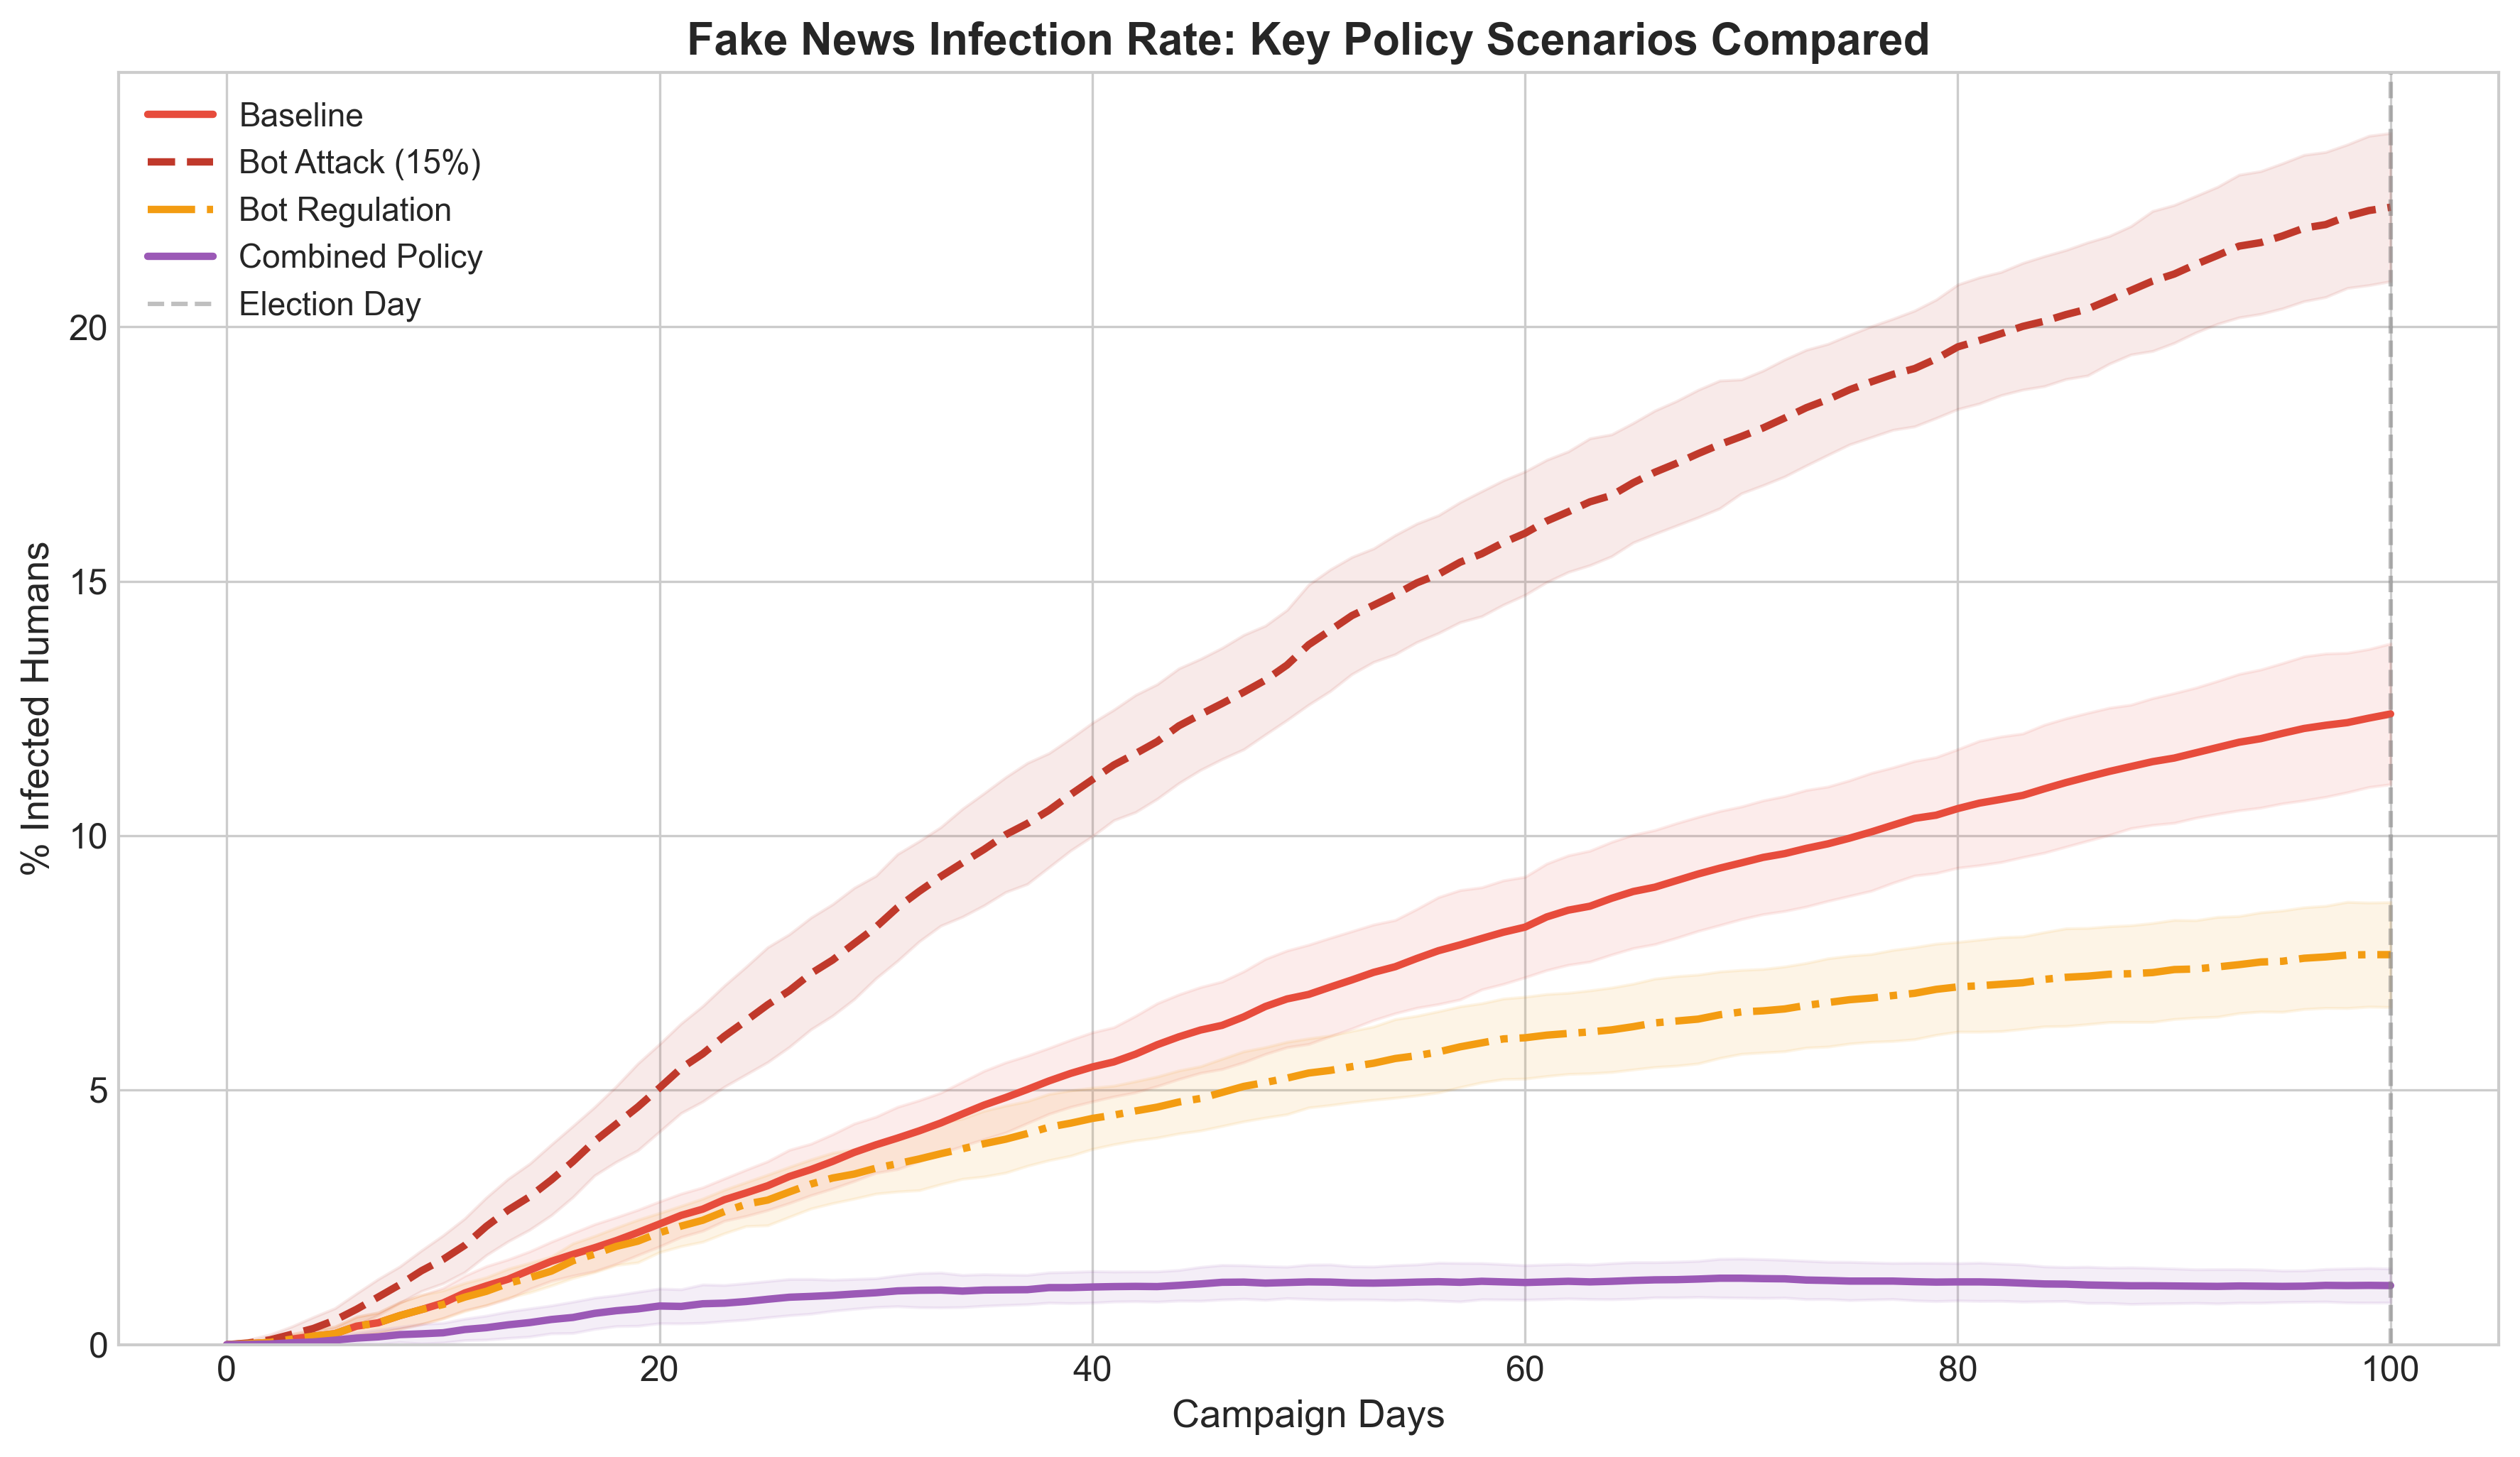
\includegraphics[width=\textwidth]{figures/fig_hero_comparacao.png}
    \caption{Taxa de infecção nos quatro cenários-chave (Brasil). Médias sobre 30 replicações; bandas = $\pm 1$ DP.}
    \label{fig:hero}
\end{figure}

\begin{table}[H]
\centering
\begin{tabular}{lccl}
\toprule
\textbf{Intervenção} & \textbf{Infectados (\%)} & \textbf{Redução} & \textbf{Mecanismo} \\
\midrule
Cenário base         & $12{,}4 \pm 1{,}4$ & ---     & --- \\
Ataque de bots (15\%)& $22{,}3 \pm 1{,}5$ & $+80\%$ & Amplificação \\
Verific.\ de fatos   & $6{,}1 \pm 1{,}0$  & $-51\%$ & $I \to R$ \\
Educação midiática   & $4{,}6 \pm 0{,}7$  & $-63\%$ & $S \to V$ \\
Regulação de bots    & $7{,}7 \pm 1{,}0$  & $-38\%$ & Remove fonte \\
\textbf{Combinado}   & $\mathbf{1{,}2 \pm 0{,}3}$ & $\mathbf{-90{,}3\%}$ & Sinergias \\
\bottomrule
\end{tabular}
\caption{Eficácia das intervenções no dia da eleição (média $\pm$ DP, $n=30$, Brasil).}
\label{tab:interventions}
\end{table}

A política combinada produz redução de 90,3\%. Sob independência multiplicativa, a redução esperada seria $\approx 88{,}8\%$; o valor observado (90,3\%) indica sinergias moderadas. Formalmente, $R_0^{\text{comb}} = 0{,}31 < 1$ (Apêndice~\ref{app:proofs}).

\subsection{Impacto Eleitoral}

A margem crítica $M_c = 2 \cdot P_{\text{flip}} \cdot q_B \cdot I(T)$, onde $P_{\text{flip}} = 12\%$ (probabilidade condicional de mudança $B \to A$ dado infectado) e $q_B = 52\%$ (fração de infectados alinhados a $B$), ambos estimados do ABM. No cenário base: $M_c = 1{,}55\%$. No ataque: $M_c = 2{,}78\%$ --- eleições disputadas tornam-se vulneráveis. Com a política combinada: $M_c = 0{,}15\%$ --- reversão virtualmente impossível (Teorema~\ref{thm:reversal}).

\subsection{Resultados Cross-Country}

\begin{table}[H]
\centering
\footnotesize
\resizebox{\textwidth}{!}{%
\begin{tabular}{llrrrrrrrrrr}
\toprule
\textbf{Cenário} & \textbf{Métrica} & \textbf{BR} & \textbf{MX} & \textbf{AR} & \textbf{CO} & \textbf{CL} & \textbf{PE} & \textbf{VE} & \textbf{EC} & \textbf{BO} & \textbf{UY} \\
\midrule
Base & Infect.\ (\%) & $12,4{\pm}1,4$ & $27,7{\pm}1,1$ & $9,0{\pm}1,0$ & $25,9{\pm}1,8$ & $4,1{\pm}0,6$ & $18,8{\pm}1,4$ & $47,1{\pm}2,0$ & $18,7{\pm}1,2$ & $29,3{\pm}2,1$ & $1,3{\pm}0,4$ \\
Ataque & Infect.\ (\%) & $20,9{\pm}1,4$ & $38,5{\pm}2,3$ & $16,2{\pm}1,1$ & $40,4{\pm}2,1$ & $7,6{\pm}1,2$ & $31,1{\pm}1,6$ & $53,3{\pm}2,1$ & $31,1{\pm}1,9$ & $45,2{\pm}2,1$ & $2,4{\pm}0,6$ \\
Combinado & Infect.\ (\%) & $1,2{\pm}0,3$ & $3,0{\pm}0,8$ & $0,7{\pm}0,3$ & $3,0{\pm}0,7$ & $0,3{\pm}0,1$ & $1,8{\pm}0,5$ & $6,7{\pm}1,0$ & $1,7{\pm}0,4$ & $3,5{\pm}0,7$ & $0,1{\pm}0,2$ \\
\bottomrule
\end{tabular}%
}
\caption{Taxas de infecção no dia da eleição por país e cenário (média $\pm$ DP, 30 replicações).}
\label{tab:crosscountry}
\end{table}

Três padrões emergem: (1) a política combinada é universalmente eficaz (86--93\% de redução em todos os 10 países); (2) intervenções individuais dependem do contexto nacional (educação midiática é mais eficaz em países com educação base já moderada --- Argentina e Uruguai --- do que na Venezuela, onde fonte persistente de bots limita o efeito a $-45\%$); (3) ataques de bots amplificam vulnerabilidade de forma não uniforme, com ``efeito teto'' nos países de alta infecção base.

\begin{figure}[H]
    \centering
    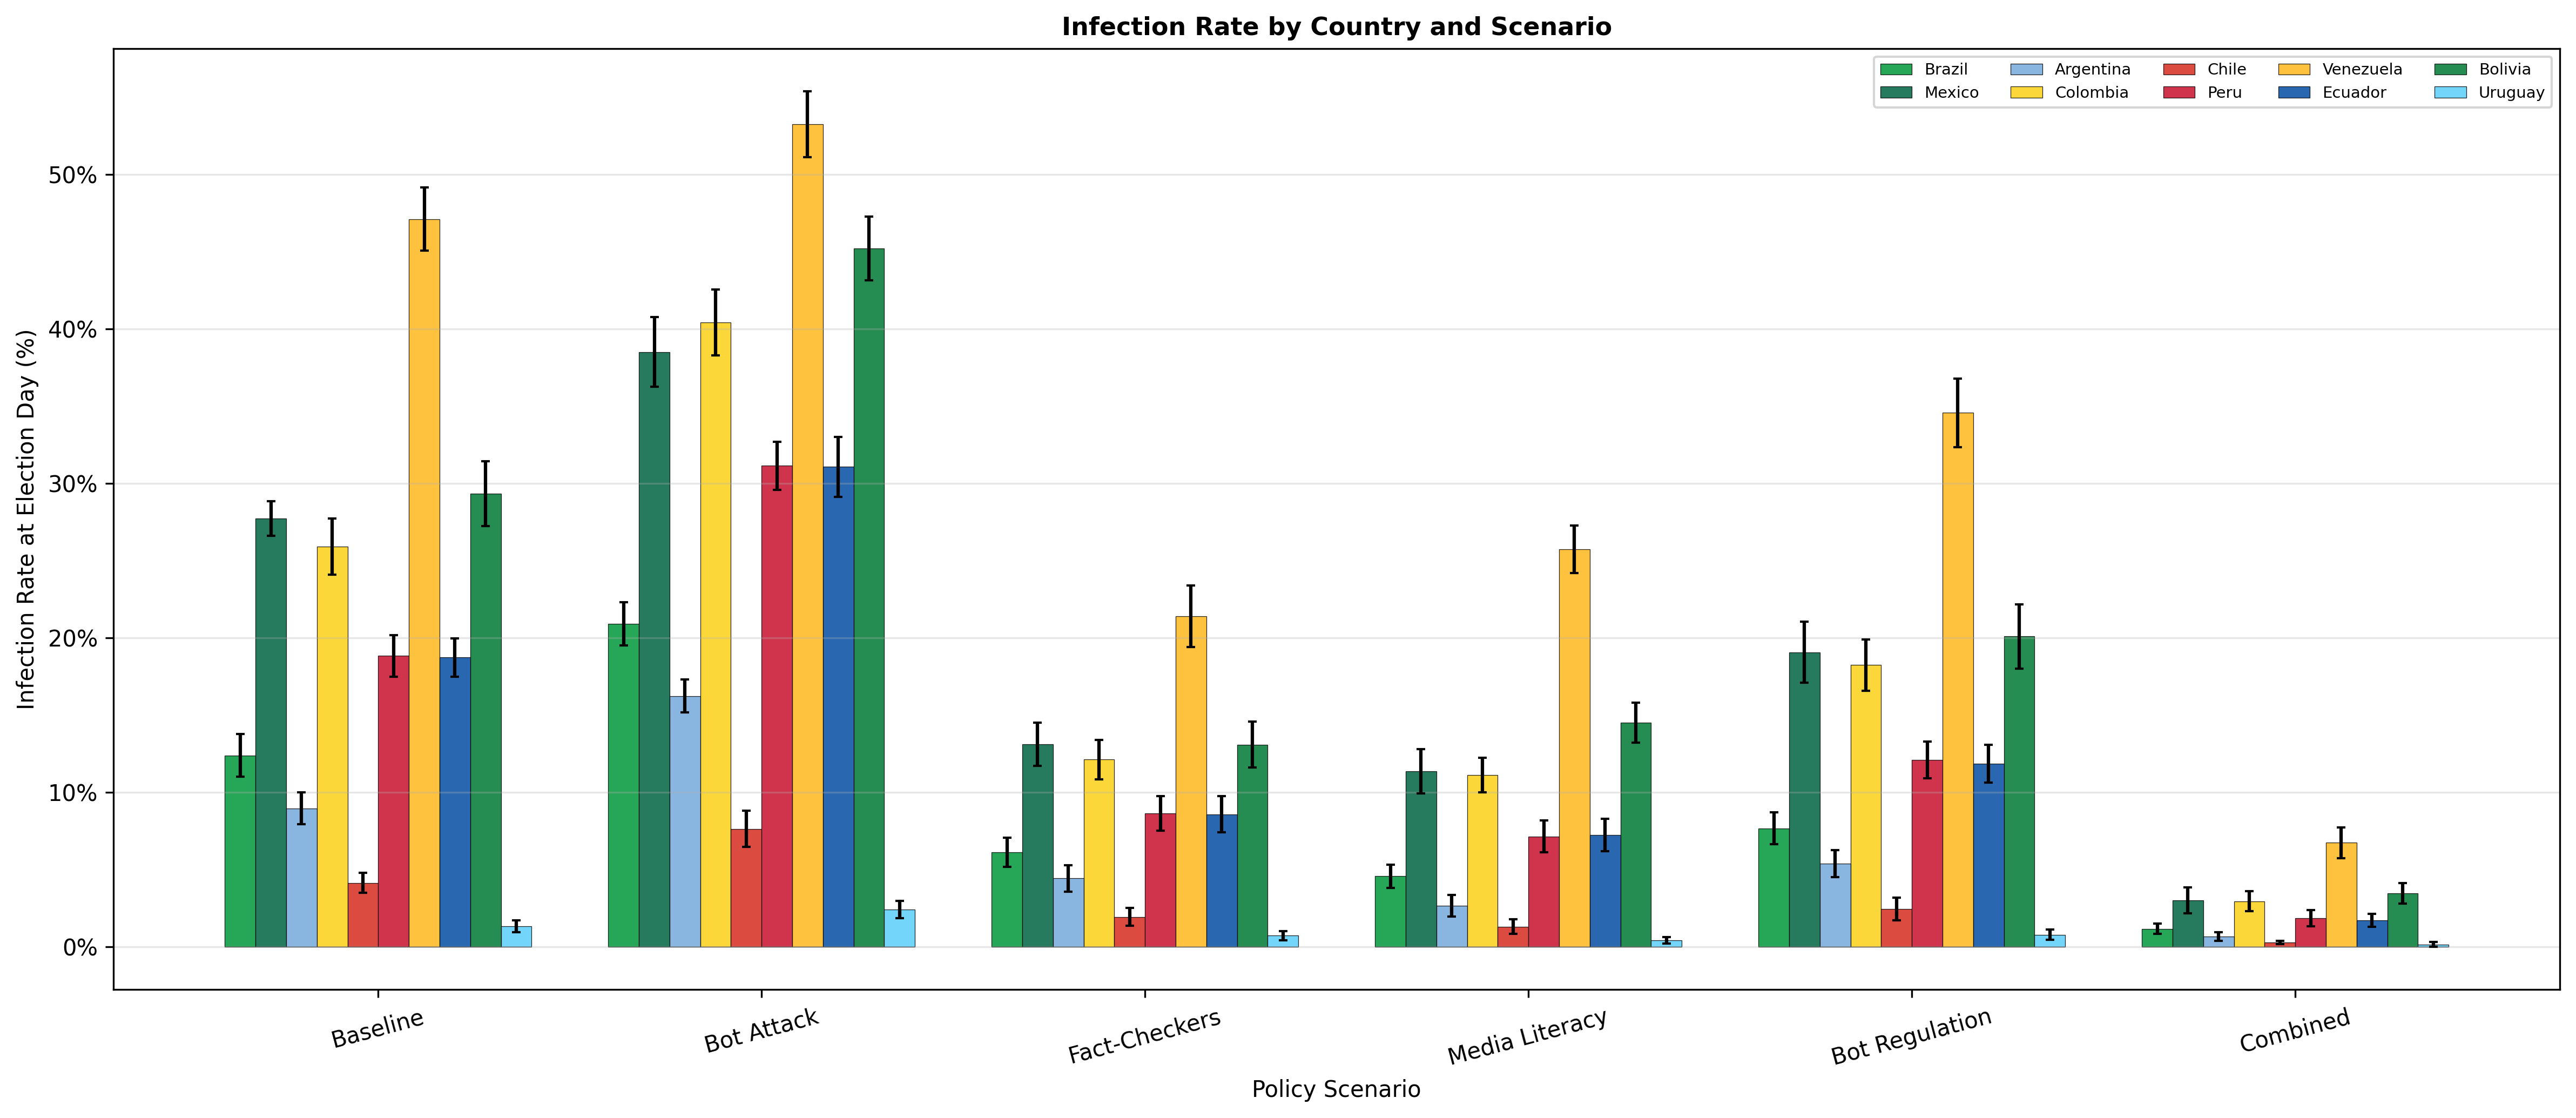
\includegraphics[width=\textwidth]{figures_countries/fig_infection_comparison.png}
    \caption{Taxa de infecção no dia da eleição por país e cenário (média $\pm$ DP, 30 replicações).}
    \label{fig:crosscountry_comparison}
\end{figure}

% ============================================================
\section{Comparação Campo Médio vs.\ ABM}
\label{sec:comparison}

Três vias de comparação: EDO canônica ($\beta = 0{,}3$, bots como condição inicial), EDO com bots como fonte permanente ($\beta_{\text{SEIR}} = 0{,}08$, $I_B = 7\%$ constante) e ABM. A EDO canônica prevê $I(100) = 2{,}0\%$; a EDO com bots produz $I_h(100) \approx 1{,}1\%$; o ABM alcança $I_{\text{hum}}(100) \approx 12{,}4\%$. A divergência de 11,3~pp tem quatro causas: (1) bots como fonte permanente vs.\ condição inicial; (2) desigualdade de Jensen pela heterogeneidade; (3) hubs da rede livre de escala; (4) estocasticidade intrínseca do ABM \citep{pastor2001epidemic}.

% ============================================================
\section{Discussão}
\label{sec:discussion}

A política combinada --- educação midiática como vacinação cognitiva, verificação de fatos como tratamento curativo e regulação de bots como eliminação da fonte --- produz reduções de 86--93\% em todos os dez países. Nenhuma intervenção isolada é suficiente. No Brasil, $R_0^{\text{hum}} \approx 0{,}71 < 1$: os bots são condição necessária para o estado endêmico, resultado que se generaliza a 8 dos 10 países. Venezuela e Bolívia são regimes de fronteira onde a transmissão humano-humano pode se sustentar --- mas mesmo nesses casos a política combinada reduz a infecção abaixo da margem crítica eleitoral.

O achado de que bots são necessários para a desinformação endêmica na maioria dos contextos implica que a regulação de plataformas --- especialmente a detecção e remoção de contas automatizadas --- é o elo mais alavancado da cadeia de intervenção. A educação midiática é complementar, não substituta: é mais eficaz em contextos de menor saturação. Em países dominados pelo WhatsApp (Brasil, México, Colômbia), intervenções compatíveis com criptografia (limites de encaminhamento, verificação de fatos baseada em comunidades) merecem ênfase.

\paragraph{Validação qualitativa.} O modelo prevê corretamente o Uruguai como país menos vulnerável (1,3\%, controle natural); identifica o plebiscito colombiano de 2016 (margem 0,43\%) como vulnerável ($M_c = 3{,}23\%$ base); e prevê margens críticas com política combinada abaixo das margens históricas de todos os países.

% ============================================================
\section{Limitações}
\label{sec:limitations}

\begin{itemize}[noitemsep]
    \item \textbf{Crenças unidimensionais.} $x \in [-1,+1]$ não captura multidimensionalidade de cenários políticos reais.
    \item \textbf{Rede estática.} Topologia BA fixada na inicialização; redes reais evoluem ao longo da campanha.
    \item \textbf{Escala e algoritmos de recomendação.} $N = 1{.}000$ é modesto para fenômenos nacionais; algoritmos de recomendação não implementados.
    \item \textbf{Parâmetros eleitorais constantes.} $P_{\text{flip}} = 12\%$ e $q_B = 52\%$ calibrados no Brasil e aplicados uniformemente; validação por país é prioridade para trabalhos futuros.
    \item \textbf{Incerteza Tier~3.} Para Peru, Venezuela, Equador, Bolívia e Uruguai, bandas de sensibilidade (Apêndice~\ref{app:sensitivity}) devem ser consultadas antes de uso normativo das estimativas.
\end{itemize}

% ============================================================
\section{Conclusão}
\label{sec:conclusion}

Este artigo integrou dinâmica SEIR informacional, heterogeneidade cognitiva, topologia de rede livre de escala e dinâmica eleitoral em um único arcabouço formal, com demonstrações matemáticas completas (conservação, positividade, estabilidade, convergência) verificadas independentemente via SymPy e Wolfram Language.

A principal conclusão teórica é que $R_0^{\text{hum}} < 1$ em 8 dos 10 países latino-americanos estudados: sem bots, a desinformação eleitoral não constitui epidemia autossustentável. Exceções --- Venezuela (1,15) e Bolívia (1,02) no ponto central, com México e Colômbia cruzando o limiar nas bandas superiores --- definem um gradiente de fronteira regime-dependente. A principal conclusão prática é que somente a política combinada reduz $R_0^{\text{comb}}$ abaixo de 1 e a margem crítica eleitoral abaixo da margem histórica mais apertada de cada país --- inclusive na Venezuela.

Trabalhos futuros incluem análise de sensibilidade global com índices de Sobol \citep{saltelli2008global}, redes dinâmicas com algoritmos de recomendação, calibração com dados primários de autoridades eleitorais nacionais (TSE, INE, CNE), e investigação empírica aprofundada dos casos-limite venezuelano e boliviano.

% ============================================================
\bibliographystyle{apalike}
\bibliography{references}

% ============================================================
\appendix

% ============================================================
\section{Provas Formais}
\label{app:proofs}

\begin{teorema}[Conservação da população]
Para todo $t \geq 0$: $S(t) + E(t) + I(t) + R(t) + V(t) = 1$.
\end{teorema}
\begin{proof}
Soma das cinco equações \eqref{eq:dS}--\eqref{eq:dV}: todos os termos se cancelam aos pares.
\end{proof}

\begin{lema}[Positividade]
Se compartimentos iniciais são não-negativos e somam 1, então são não-negativos para todo $t \geq 0$.
\end{lema}
\begin{proof}
Verifica-se que cada variável tem derivada $\geq 0$ quando atinge zero: $dS/dt|_{S=0} = \delta R \geq 0$; análogo para $E, I, R, V$.
\end{proof}

\begin{lema}[Sem propagação sem fonte]
Se $I(0) = E(0) = 0$, então $I(t) = E(t) = 0$ para todo $t$.
\end{lema}
\begin{proof}
Com $E(0)=I(0)=0$: $dE/dt = dI/dt = 0$. Pela unicidade de Picard-Lindelöf, $E(t)=I(t)=0$.
\end{proof}

\begin{teorema}[Estabilidade do Equilíbrio Livre de Doença]
O ELD $(S^*, 0, 0, 0, V^*)$ é localmente assintoticamente estável se e somente se $R_0^{\text{eff}} \cdot S^* < 1$.
\end{teorema}
\begin{proof}
Jacobiano do subsistema $(E,I)$ em torno do ELD: $\mathbf{J} = \bigl(\begin{smallmatrix}-(\sigma+\gamma_e) & \beta S^*\\ \sigma & -\gamma\end{smallmatrix}\bigr)$. Por Routh-Hurwitz: $\det(\mathbf{J}) = \gamma(\sigma+\gamma_e)(1-R_0^{\text{eff}}S^*) > 0 \Leftrightarrow R_0^{\text{eff}}S^* < 1$.
\end{proof}

\begin{teorema}[Convergência de crenças]
\label{thm:convergence}
Após $n$ infecções por fake news com orientação $o_k$: $x^{(n)} = o_k + (x^{(0)} - o_k)(1-\mu)^n$.
\end{teorema}
\begin{proof}
Recorrência geométrica $y^{(n+1)} = (1-\mu)y^{(n)}$ com $y^{(n)} = x^{(n)}-o_k$.
\end{proof}

\begin{teorema}[Reversão eleitoral]
\label{thm:reversal}
Uma eleição com margem $M$ pode ser revertida se e somente se $M < M_c = 2 \cdot p_I \cdot q_B \cdot P_{\text{flip}}$.
\end{teorema}
\begin{proof}
$N_B = N(1+M)/2$, $N_A = N(1-M)/2$. Votos deslocados: $\Delta = N \cdot p_I \cdot q_B \cdot P_{\text{flip}}$. Reversão quando $2\Delta > NM$.
\end{proof}

\begin{proposicao}[Extinção sob política combinada]
Com $\bar{e} = 0{,}7$: $\beta_{\text{SEIR}}^{\text{comb}} \approx 0{,}034$; $R_0^{\text{comb}} = 0{,}034 \times 0{,}2 / (0{,}1 \times 0{,}22) \approx 0{,}31 < 1$.
\end{proposicao}

% ============================================================
\section{Validação Estatística}
\label{app:statistics}

Comparações entre cenários usam teste de Mann-Whitney $U$ (não paramétrico). Com 6 cenários, 15 comparações pareadas; correção de Bonferroni: $\alpha_{\text{adj}} = 0{,}05/15 = 0{,}0033$. Todos os $p < 0{,}001$ --- bem abaixo do limiar. Correlação biserial de postos $> 0{,}8$ em todas as comparações envolvendo a política combinada.

Para 10 países: $10 \times 5 = 50$ comparações com $\alpha_{\text{Bonf}} = 0{,}001$. Todas as 50 comparações são significativas após Bonferroni, com $|d| \geq 0{,}8$ em todas (Cohen grande).

% ============================================================
\section{Análise de Sensibilidade (Tier~3)}
\label{app:sensitivity}

\begin{table}[H]
\centering
\small
\begin{tabular}{lcccc}
\toprule
\textbf{País} & \textbf{Central} & \textbf{Intervalo} & \textbf{Desvio máx.} & \textbf{Desvio rel.} \\
\midrule
Peru     & $18,3\%$ & $[12,5,\,22,6]$ & $5,8$pp & $32\%$ \\
Venezuela& $47,6\%$ & $[40,7,\,50,9]$ & $6,8$pp & $14\%$ \\
Equador  & $18,8\%$ & $[12,5,\,22,9]$ & $6,3$pp & $33\%$ \\
Bolívia  & $29,9\%$ & $[21,4,\,35,7]$ & $8,4$pp & $28\%$ \\
Uruguai  & $1,4\%$  & $[0,3,\,2,4]$   & $1,1$pp & $78\%$ \\
\bottomrule
\end{tabular}
\caption{Sensibilidade para países Tier~3 (cenário base). Perturbações: bots $\pm 3$pp, educação $\pm 0{,}10$, viralidade $\pm 0{,}05$. Ranking qualitativo preservado em todas as variações.}
\label{tab:sensitivity_tier3}
\end{table}

% ============================================================
\section{Parâmetros por País}
\label{app:countryparams}

\begin{table}[H]
\centering
\footnotesize
\resizebox{\textwidth}{!}{%
\begin{tabular}{lcccccccccc}
\toprule
\textbf{Parâmetro} & \textbf{BR} & \textbf{MX} & \textbf{AR} & \textbf{CO} & \textbf{CL} & \textbf{PE} & \textbf{VE} & \textbf{EC} & \textbf{BO} & \textbf{UY} \\
\midrule
Tier de dados    & 1          & 2          & 2          & 2          & 2          & 3          & 3          & 3          & 3          & 3          \\
Bots (\%)        & 7\%        & 12\%       & 9\%        & 10\%       & 6\%        & 8\%        & 15\%       & 8\%        & 9\%        & 4\%        \\
VF (\%)          & 3\%        & 2\%        & 4\%        & 2\%        & 4\%        & 2\%        & 1\%        & 2\%        & 1\%        & 5\%        \\
Educ.\ midiática & 0,30       & 0,25       & 0,35       & 0,25       & 0,40       & 0,25       & 0,20       & 0,25       & 0,20       & 0,45       \\
Viralidade       & 0,21--0,28 & 0,23--0,32 & 0,19--0,27 & 0,25--0,35 & 0,18--0,25 & 0,22--0,30 & 0,26--0,38 & 0,22--0,30 & 0,24--0,33 & 0,15--0,22 \\
Credib.\         & 0,85--0,99 & 0,83--0,97 & 0,82--0,96 & 0,85--0,98 & 0,80--0,94 & 0,84--0,97 & 0,87--0,99 & 0,84--0,97 & 0,86--0,98 & 0,78--0,93 \\
$m$ (BA)         & 3          & 3          & 4          & 3          & 4          & 3          & 3          & 3          & 3          & 4          \\
Margem (\%)      & 3,28       & 0,56       & 2,68       & 0,43       & 11,74      & 0,25       & 1,49       & 4,72       & 0,50       & 1,30       \\
\bottomrule
\end{tabular}%
}
\caption{Parâmetros específicos por país e tier de dados. VF: verificadores de fatos.}
\label{tab:countryparams}
\end{table}

% ============================================================
\section{Declarações do Autor}
\label{app:author_statements}

\subsection*{Protocolo de Disseminação Científica Pós-Publicação}

Os autores comprometem-se a disseminar os resultados por meio de plataformas digitais (LinkedIn, Reddit, YouTube) em conformidade com as políticas editoriais e os termos de cessão de direitos autorais. A versão oficial publicada não será redistribuída sem autorização. Todo o material de divulgação será redigido com as próprias palavras dos autores e o acesso ao artigo completo será direcionado via DOI.

\subsection*{Declaração de Uso de Ferramentas de IA e Plataformas Colaborativas}

Em conformidade com as diretrizes do CNPq-Brasil, os autores declaram que ferramentas de IA (GLM da Zhipu AI; ChatGPT e Codex da OpenAI; Gemini do Google; Claude da Anthropic) foram utilizadas para auxiliar na redação em língua inglesa, no desenvolvimento de código em Python e Wolfram Language, na geração de figuras e tabelas, e na editoração em \LaTeX{}. Todas as derivações teóricas, a especificação do modelo, o desenho empírico e a interpretação dos resultados são de responsabilidade exclusiva dos autores.

% ============================================================
\end{document}
